\documentclass{amsart}
%DIF LATEXDIFF DIFFERENCE FILE
%DIF DEL report0.tex   Mon Apr 26 14:43:08 2021
%DIF ADD report.tex    Mon Apr 26 14:37:27 2021
\synctex=1

%=================================================================
% 
\newcount\DraftStatus  % 0 suppresses notes to selves in text
\DraftStatus=1   % TODO: set to 0 for final version
%=================================================================

%=================================================================
\usepackage{comment}
%=================================================================
%
\includecomment{JournalOnly}  
\includecomment{ConferenceOnly}  
\includecomment{TulipStyle}
%
%=================================================================
%=================================================================
% gitlatexdiff
%
%  https://gitlab.com/git-latexdiff/git-latexdiff
%=================================================================
%  git latexdiff HEAD  HEAD~5 --main templatex.tex
%  git latexdiff HEAD~1  --main templatex.tex
%  View pdf to see difference
%
%=================================================================
%
% Todo Notes for marginal comments
% 
%\newcount\DraftStatus  % 0 suppresses notes to selves in text
%\DraftStatus=1   % TODO: set to 0 for final version
\ifnum\DraftStatus=1
	\usepackage[draft,colorinlistoftodos,color=orange!30]{todonotes}
\else
	\usepackage[disable,colorinlistoftodos,color=blue!30]{todonotes}
\fi 
%\usepackage[disable]{todonotes} % notes not showed
%\usepackage[draft]{todonotes}   % notes showed
%
\makeatletter
 \providecommand\@dotsep{5}
 \def\listtodoname{List of Todos}
 \def\listoftodos{\@starttoc{tdo}\listtodoname}
 \makeatother
%
%=================================================================
%
\usepackage{color}
\newcommand{\draftnote}[3]{ 
	\todo[author=#2,color=#1!30,size=\footnotesize]{\textsf{#3}}	}
% TODO: add yourself here:
%
\newcommand{\gangli}[1]{\draftnote{blue}{GLi:}{#1}}
\newcommand{\qwu}[1]{\draftnote{red}{QWu:}{#1}}
\newcommand{\gliMarker}
	{\todo[author=GLi,size=\tiny,inline,color=blue!40]
	{Gang Li has worked up to here.}}
\newcommand{\qwuMarker}
	{\todo[author=QWu,size=\tiny,inline,color=red!40]
	{Qiong Wu has worked up to here.}}
%=================================================================

%=================================================================
%
% general packages
%  https://en.wikibooks.org/wiki/Category:Book:LaTeX
%  https://en.wikibooks.org/wiki/LaTeX/Package_Reference
%
%=================================================================
\usepackage{graphicx}
\usepackage{algorithm}
\usepackage{algorithmic}
\usepackage{breqn}
\usepackage{subcaption}
\usepackage{multirow}
\usepackage{psfrag}
\usepackage{url}
\usepackage{hyperref}
%\usepackage[colorlinks]{hyperref}
%\usepackage{cite}
\usepackage{cleveref}
\usepackage{booktabs}
\usepackage{rotating}
\usepackage{colortbl}
\usepackage{paralist}
%\usepackage{geometry}
\usepackage{epstopdf}
\usepackage{nag}
\usepackage{microtype}
\usepackage{siunitx}
\usepackage{nicefrac}
\usepackage{breakurl}
\usepackage{fontawesome}
\usepackage{xcolor}
\usepackage{multicol}
\usepackage{wrapfig}
\usepackage{todonotes}
\usepackage{tablefootnote}
\usepackage{threeparttable}
% for random text
\usepackage{lipsum}
\usepackage[english]{babel}
\usepackage[pangram]{blindtext}
% for tikz figures
\usepackage{tikz}
\usetikzlibrary{fit,positioning,arrows.meta,shapes,arrows}
%\tikzset{neuron/.style={circle,thick,fill=black!25,minimum size=17pt,inner sep=0pt},
%	input neuron/.style={neuron, draw,thick, fill=gray!30},
%	hidden neuron/.style={neuron,fill=white,draw},
%	hoz/.style={rotate=-90}}
%
%=================================================================



\begin{TulipStyle}
\usepackage[numbers]{natbib}
%=================================================================
%
% Version control information
%
%=================================================================
\usepackage{gitinfo2}
%=================================================================
\usepackage{fancyhdr}
\pagestyle{fancy}
\fancyhead{} % clear all header fields
\fancyhead[RO,LE]{\textsl{\rightmark}}
\fancyhead[LO,RE]{\ensuremath{\Rightarrow}
		\textbf{\textbf{[CONFIDENTIAL]}}\ensuremath{\Leftarrow}}
\fancyhead[CO,CE]{}
%=================================================================
\fancyfoot{} % clear all footer fields
\fancyfoot[CE,CO]{\textbf{\thepage}} 
\fancyfoot[LO,LE]{
\includegraphics[height=.9\headheight]{logos/tulip-logo.eps}
		\gitVtagn-\gitBranch\ (\gitCommitterDate)}
\fancyfoot[RO,RE]{Committed by: \textsl{\gitCommitterName}}

\setlength{\headheight}{12pt}
\renewcommand{\headrulewidth}{0.4pt}
\renewcommand{\footrulewidth}{0.4pt}
%=================================================================


%=================================================================
% for math notations
% ----------------------------------------------------------------
\usepackage{mathtools}
\usepackage{amsthm}
%
% THEOREMS -------------------------------------------------------
%
\newtheorem{thm}{Theorem}[section]
\newtheorem{cor}[thm]{Corollary}
\newtheorem{lem}[thm]{Lemma}
\newtheorem{prop}[thm]{Proposition}
\theoremstyle{definition}
\newtheorem{defn}[thm]{Definition}
\theoremstyle{remark}
\newtheorem{rem}[thm]{Remark}
\numberwithin{equation}{section}
% MATH -----------------------------------------------------------
\newcommand{\norm}[1]{\left\Vert#1\right\Vert}
\newcommand{\abs}[1]{\left\vert#1\right\vert}
\newcommand{\set}[1]{\left\{#1\right\}}
\newcommand{\Real}{\mathbb R}
\newcommand{\eps}{\varepsilon}
\newcommand{\To}{\longrightarrow}
\newcommand{\BX}{\mathbf{B}(X)}
% ----------------------------------------------------------------
\newcommand{\I}{{\cal I}}
\newcommand{\Id}{{\cal I} }
\newcommand{\Dc}{{\cal D}}
\newcommand{\J}{{\cal J}}
\newcommand{\Dn}{{\cal D}_n}
\newcommand{\Dd}{{\cal D}_n }
\renewcommand{\P}{{\cal P}}
\newcommand{\Nu}{{\cal N} }
\newcommand{\B}{{\cal B}}
\newcommand{\Bf}{{\bf B}}
\newcommand{\Y}{{\bf Y}}
\newcommand{\A}{{\cal A}}
% ----------------------------------------------------------------
\newcommand{\V}{{\cal V}}
\newcommand{\M}{{\cal M}}
\newcommand{\F}{{\cal F}}
\newcommand{\Fd}{{\cal F}}
\newcommand{\BF}{{\cal BF}_n}
\newcommand{\BFd}{{\cal BF}_n}
\newcommand{\TF}{{\cal TF}_n}
\newcommand{\TFd}{{\cal TF}_n}
%\newcommand{\G}{{\cal G}}
\newcommand{\X}{{\cal X}}
\newcommand{\E}{{\cal E}}
\newcommand{\K}{{\cal K}}
\newcommand{\T}{{\cal T}_n}
\renewcommand{\H}{{\cal H}}
% ----------------------------------------------------------------
\newtheorem{Remark}{Remark}
\newtheorem{proposition}{Proposition}
\newtheorem{theorem}{Theorem}
\newtheorem{lemma}{Lemma}
\newtheorem{corollary}{Corollary}
\newtheorem{example}{Example}
\newtheorem{definition}{Definition}
\newtheorem{Algorithms}{Algorithm}
% ----------------------------------------------------------------
\newcommand{\bu}{{\mathbf 1} }
\newcommand{\bo}{{\mathbf 0} }
\newcommand{\N}{\mbox{{\sl l}}\!\mbox{{\sl N}}}
% ----------------------------------------------------------------
\def\uint{[0,1]}
\def\proof{{\scshape Proof}. \ignorespaces}
\def\endproof{{\hfill \vbox{\hrule\hbox{%
   \vrule height1.3ex\hskip1.0ex\vrule}\hrule
  }}\par}
%
%=================================================================

\hypersetup
{
    pdfauthor={\gitAuthorName},
    pdfsubject={TULIP Lab},
    pdftitle={},
    pdfkeywords={TULIP Lab, Data Science},
%	bookmarks=true,  
}

\end{TulipStyle}




%=================================================================
%
%DIF PREAMBLE EXTENSION ADDED BY LATEXDIFF
%DIF UNDERLINE PREAMBLE %DIF PREAMBLE
\RequirePackage[normalem]{ulem} %DIF PREAMBLE
\RequirePackage{color}\definecolor{RED}{rgb}{1,0,0}\definecolor{BLUE}{rgb}{0,0,1} %DIF PREAMBLE
\providecommand{\DIFadd}[1]{{\protect\color{blue}\uwave{#1}}} %DIF PREAMBLE
\providecommand{\DIFdel}[1]{{\protect\color{red}\sout{#1}}}                      %DIF PREAMBLE
%DIF SAFE PREAMBLE %DIF PREAMBLE
\providecommand{\DIFaddbegin}{} %DIF PREAMBLE
\providecommand{\DIFaddend}{} %DIF PREAMBLE
\providecommand{\DIFdelbegin}{} %DIF PREAMBLE
\providecommand{\DIFdelend}{} %DIF PREAMBLE
\providecommand{\DIFmodbegin}{} %DIF PREAMBLE
\providecommand{\DIFmodend}{} %DIF PREAMBLE
%DIF FLOATSAFE PREAMBLE %DIF PREAMBLE
\providecommand{\DIFaddFL}[1]{\DIFadd{#1}} %DIF PREAMBLE
\providecommand{\DIFdelFL}[1]{\DIFdel{#1}} %DIF PREAMBLE
\providecommand{\DIFaddbeginFL}{} %DIF PREAMBLE
\providecommand{\DIFaddendFL}{} %DIF PREAMBLE
\providecommand{\DIFdelbeginFL}{} %DIF PREAMBLE
\providecommand{\DIFdelendFL}{} %DIF PREAMBLE
%DIF LISTINGS PREAMBLE %DIF PREAMBLE
\RequirePackage{listings} %DIF PREAMBLE
\RequirePackage{color} %DIF PREAMBLE
\lstdefinelanguage{DIFcode}{ %DIF PREAMBLE
%DIF DIFCODE_UNDERLINE %DIF PREAMBLE
  moredelim=[il][\color{red}\sout]{\%DIF\ <\ }, %DIF PREAMBLE
  moredelim=[il][\color{blue}\uwave]{\%DIF\ >\ } %DIF PREAMBLE
} %DIF PREAMBLE
\lstdefinestyle{DIFverbatimstyle}{ %DIF PREAMBLE
	language=DIFcode, %DIF PREAMBLE
	basicstyle=\ttfamily, %DIF PREAMBLE
	columns=fullflexible, %DIF PREAMBLE
	keepspaces=true %DIF PREAMBLE
} %DIF PREAMBLE
\lstnewenvironment{DIFverbatim}{\lstset{style=DIFverbatimstyle}}{} %DIF PREAMBLE
\lstnewenvironment{DIFverbatim*}{\lstset{style=DIFverbatimstyle,showspaces=true}}{} %DIF PREAMBLE
%DIF END PREAMBLE EXTENSION ADDED BY LATEXDIFF

\begin{document}
%
%=================================================================
%
\title[Report]{Report}%

\author{Bing Liu}
\address[A.~1]{School of Computer Science,\\ 
Jilin University, ChangChun 130012, China}%
\email[A.~1]{bliu@tulip.academy}


%\thanks{Thanks to \ldots}%
\subjclass{Artificial Intelligence}%
\date{\gitAuthorDate}%

%
\begin{abstract}
In this report, liubing liubing will talk about my work achievement. After systematically learning latex and Git, mastering its basic operations, and at the same time completing python learning, and I test the learning results by completing a predictive kaggle question. The following is a detailed introduction about the kaggle competition of Bike Sharing Demand.
\end{abstract}

\keywords{Machine Learning, Data Mining, python, latex, git}%



\begin{abstract}
	In this report, I will talk about my work \DIFdelbegin \DIFdel{. After }\DIFdelend \DIFaddbegin \DIFadd{achievement. After systematically }\DIFaddend learning latex and Git, mastering its basic operations, and at the same time completing python learning, and I test \DIFdelbegin \DIFdel{myself }\DIFdelend \DIFaddbegin \DIFadd{the learning results }\DIFaddend by completing a predictive kaggle question. The following is a detailed introduction about the kaggle competition \DIFaddbegin \DIFadd{of Bike Sharing Demand}\DIFaddend .
\end{abstract}

\keywords{Machine Learning, Data Mining, python, latex, git}%


\maketitle
\tableofcontents

\newpage
%=================================================================

%%=================================================================
\section{Introduction}\label{sec-intro}

\subsection{Background}
The bicycle sharing system is a way of renting bicycles. Through the network of kiosk locations throughout the city, membership is automatically obtained, and the process of renting and returning bicycles. Using these systems, people can rent a bicycle from one place and return it to other places as needed. Currently, there are more than 500 bike sharing programs worldwide.\\

\subsection{Target}
In this competition, participants are asked to combine historical usage patterns with weather data in order to forecast bike rental demand in the Capital Bikeshare program in Washington, D.C.

\section{Data} \label{sec-preliminaries}
\subsection{Data Description}
The competition provide hourly rental data spanning two years.the training set is comprised of the first 19 days of each month, while the test set is the 20th to the end of the month. The taskis to predict the total count of bikes rented during each hour covered by the test set, using only information available prior to the rental period.\\

\begin{itemize}
	\smallskip
	\item \textbf{train.csv} -- it contains 10886 rows and 12 columns. Each row represents bike rental data for a certain hour. Each column indicates the current conditions
	\smallskip
	\item \textbf{test.csv} -- it contains 6493 rows and 9 columns. Compared with the train data, there are fewer "casual","registered" and "count" columns.
	\smallskip
	\item \textbf{sampleSubmission.csv} -- it clarifies the data submission format. It just contains 2 columns that is "datetime" and "count".
\end{itemize}

\subsection{Data Fields}
The following is a detailed introduction of the data for each attributes.\\
\begin{tabular}{c| c c c c }
	\toprule
	\textbf{column} & \textbf{description}  \\
	\midrule
	$datetime$ &  {hourly date + timestamp }\\
	$season$ &  {1 = spring, 2 = summer, 3 = fall, 4 = winter} \\
	$holiday$ &  {whether the day is considered a holiday} \\
	$workingday$ &  {whether the day is neither a weekend nor holiday} \\
	$weather$ &  {1=clear, 2=mist + cloudy, 3=light snow, 4=heavy rain} \\
	$temp$ & {temperature in Celsius} \\
	$atemp$ & {"feels like" temperature in Celsius} \\
	$humidity$ & {relative humidity} \\
	$windspeed$ & {wind speed} \\
	$casual$ & {number of non-registered user rentals initiated} \\
	$registered$ & {number of registered user rentals initiated} \\
	$count$ & {number of total rentals} \\
	\bottomrule
\end{tabular}

\subsection{Missing Values Analysis}
I use "missingno" to visualize missing value in the dataset, Luckily the dataset do not has any missing value.\\
\begin{figure}[htbp]
	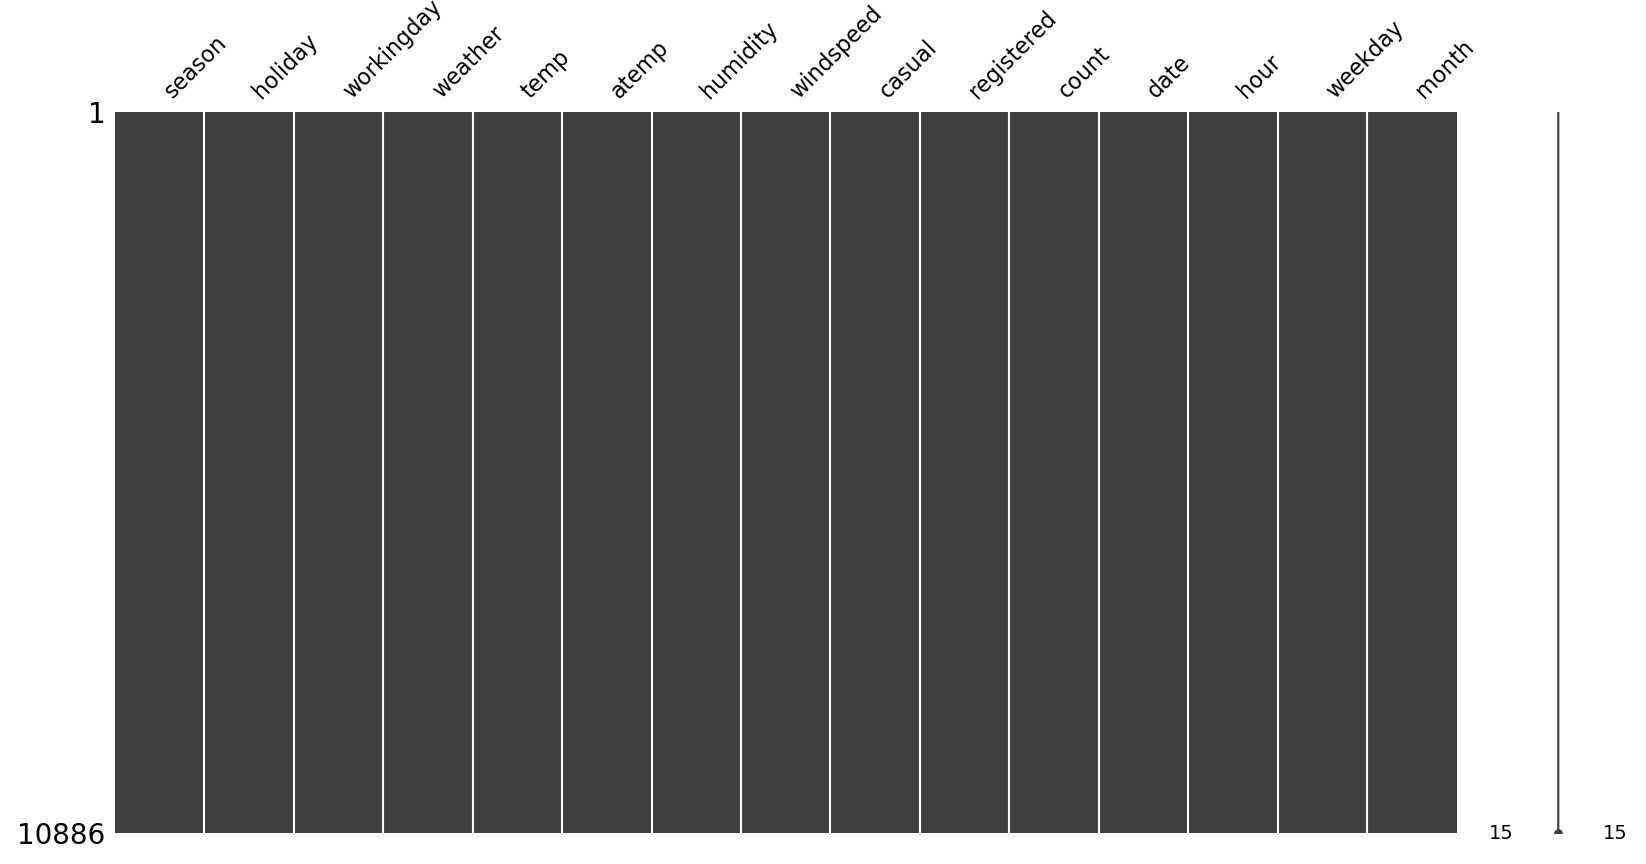
\includegraphics[scale=0.3]{./figure/Figure_1.eps}
	\caption{Missing values analysis}
\end{figure}

\subsection{Outliers Analysis}
1:Spring season has got relatively lower count. \\
2:The boxplot with "Hour Of The Day" is quiet interesting.The median value are relatively higher at 7AM to 8AM and 5PM to 6PM.\\
3:Most of the outlier points are mainly contributed from "Working Day" than "Non Working Day". 
\begin{figure}[htbp]
	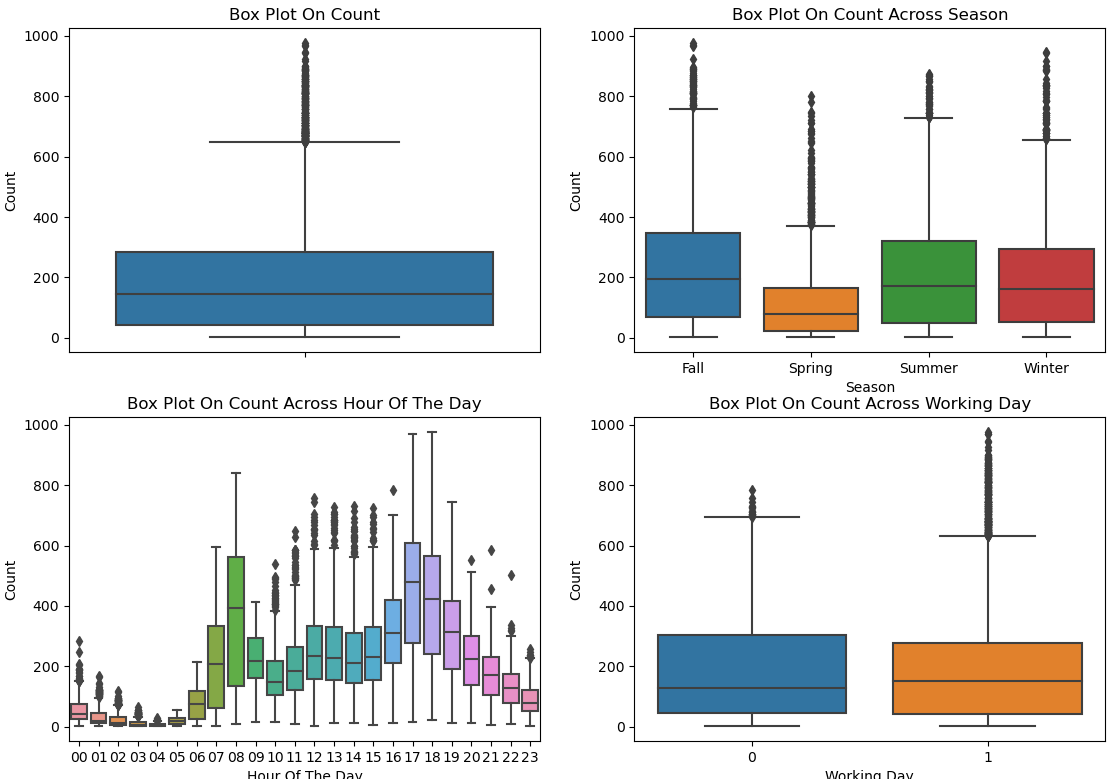
\includegraphics[scale=0.4]{./figure/Figure_2.eps}
	\caption{Outliers analysis}
\end{figure}

\subsection{Correlation Analysis}
1:temp and humidity features has got positive and negative correlation with count respectively. the count variable has got little dependency on "temp" and "humidity". \\
2:"Casual" and "Registered" are also not taken into account since they are leakage variables in nature and need to dropped during model building. \\
3:windspeed is not gonna be really useful numerical feature.
\begin{figure}[htbp]
	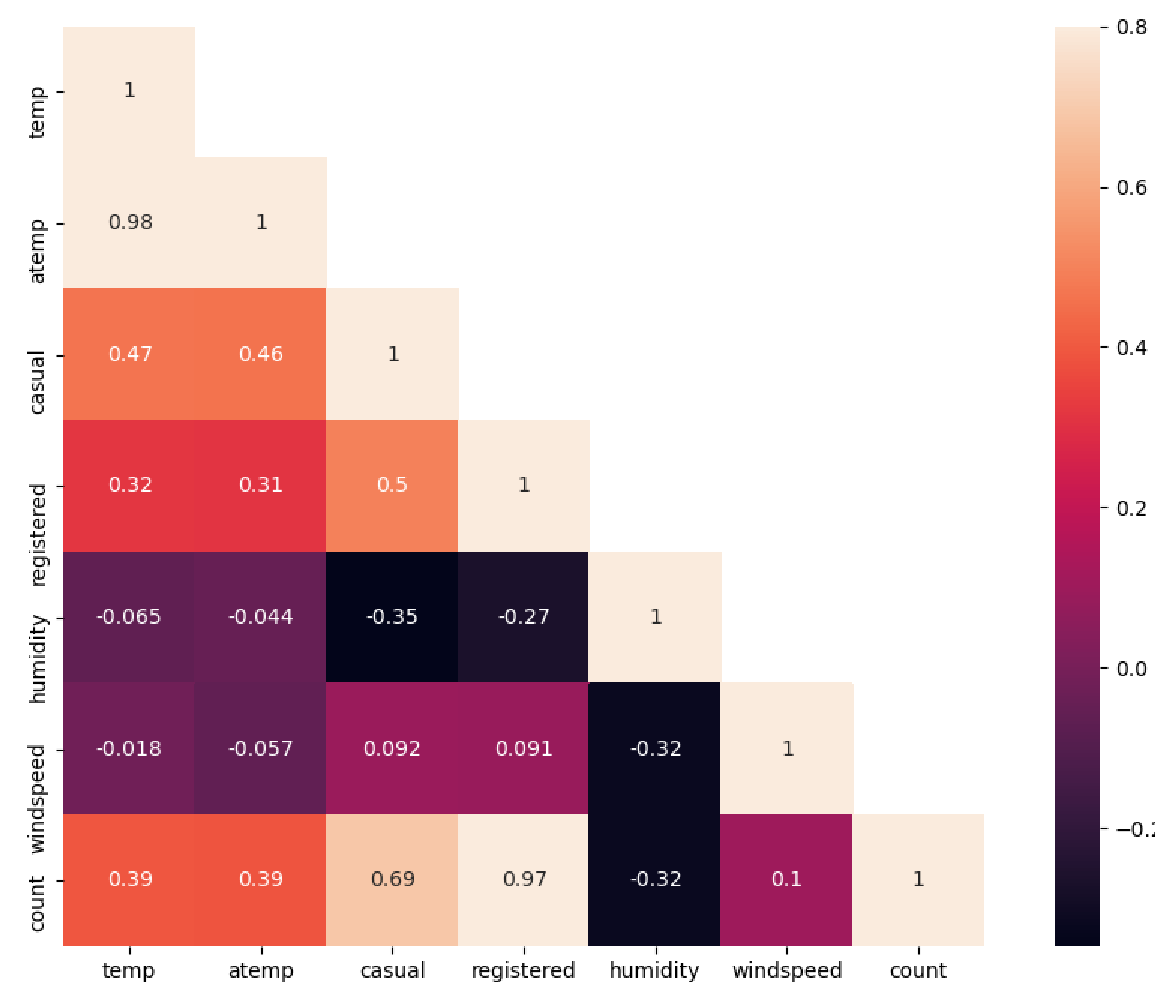
\includegraphics[scale=0.5]{./figure/Figure_3.eps}
	\caption{Correlation Analysis I}
\end{figure}

Regression plot in seaborn is one useful way to depict the relationship between two features. Here we consider "count" vs "temp", "humidity", "windspeed".
\begin{figure}[htbp]
	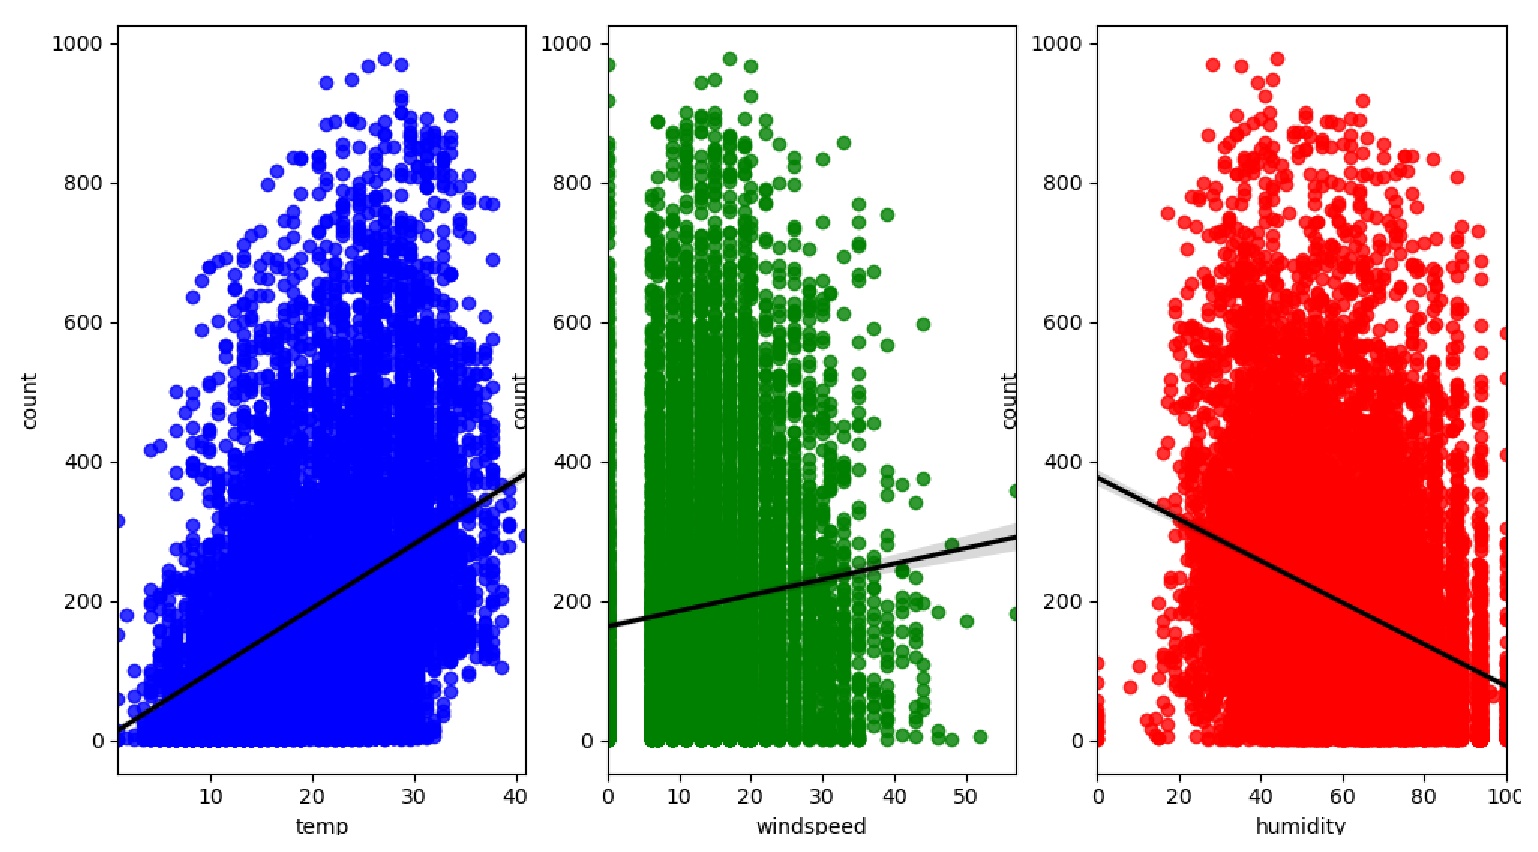
\includegraphics[scale=0.5]{./figure/Figure_4.eps}
	\caption{Correlation Analysis II}
\end{figure}

\subsection{Visualizing Distribution Of Data}
 It is desirable to have Normal distribution as most of the machine learning techniques require dependent variable to be Normal. One possible solution is to take log transformation on "count" variable after removing outlier data points.
\begin{figure}[htbp]
	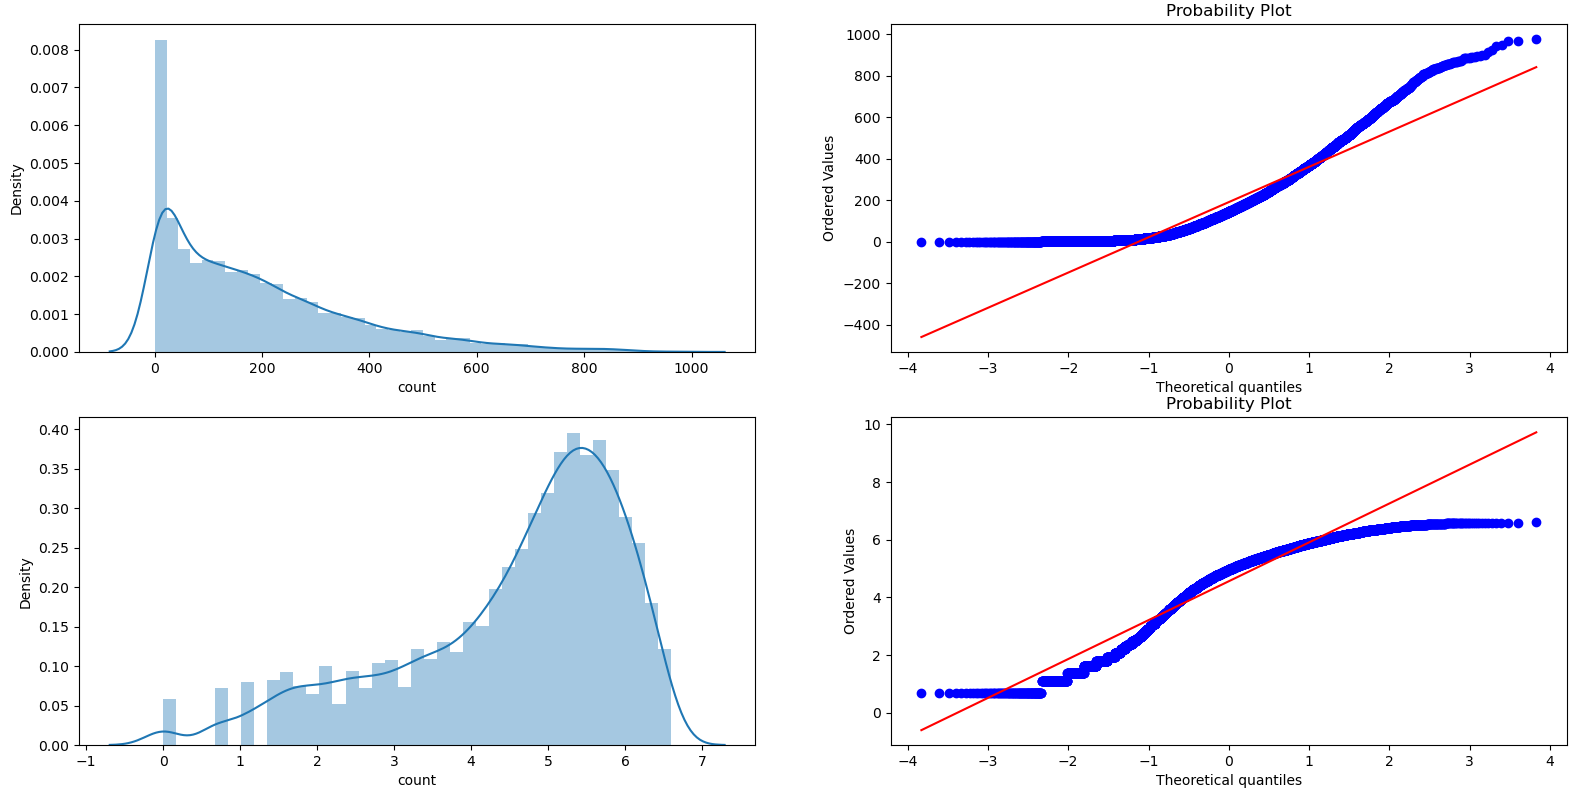
\includegraphics[scale=0.3]{./figure/Figure_5.eps}
	\caption{Visualizing Distribution Of Data}
\end{figure}

\subsection{Visualizing Count}
1:It is quiet obvious that people tend to rent bike during summer season. Therefore June, July and August has got relatively higher demand for bicycle.\\
2:On weekdays more people tend to rent bicycle around 7AM-8AM and 5PM-6PM. 
\begin{figure}[htbp]
	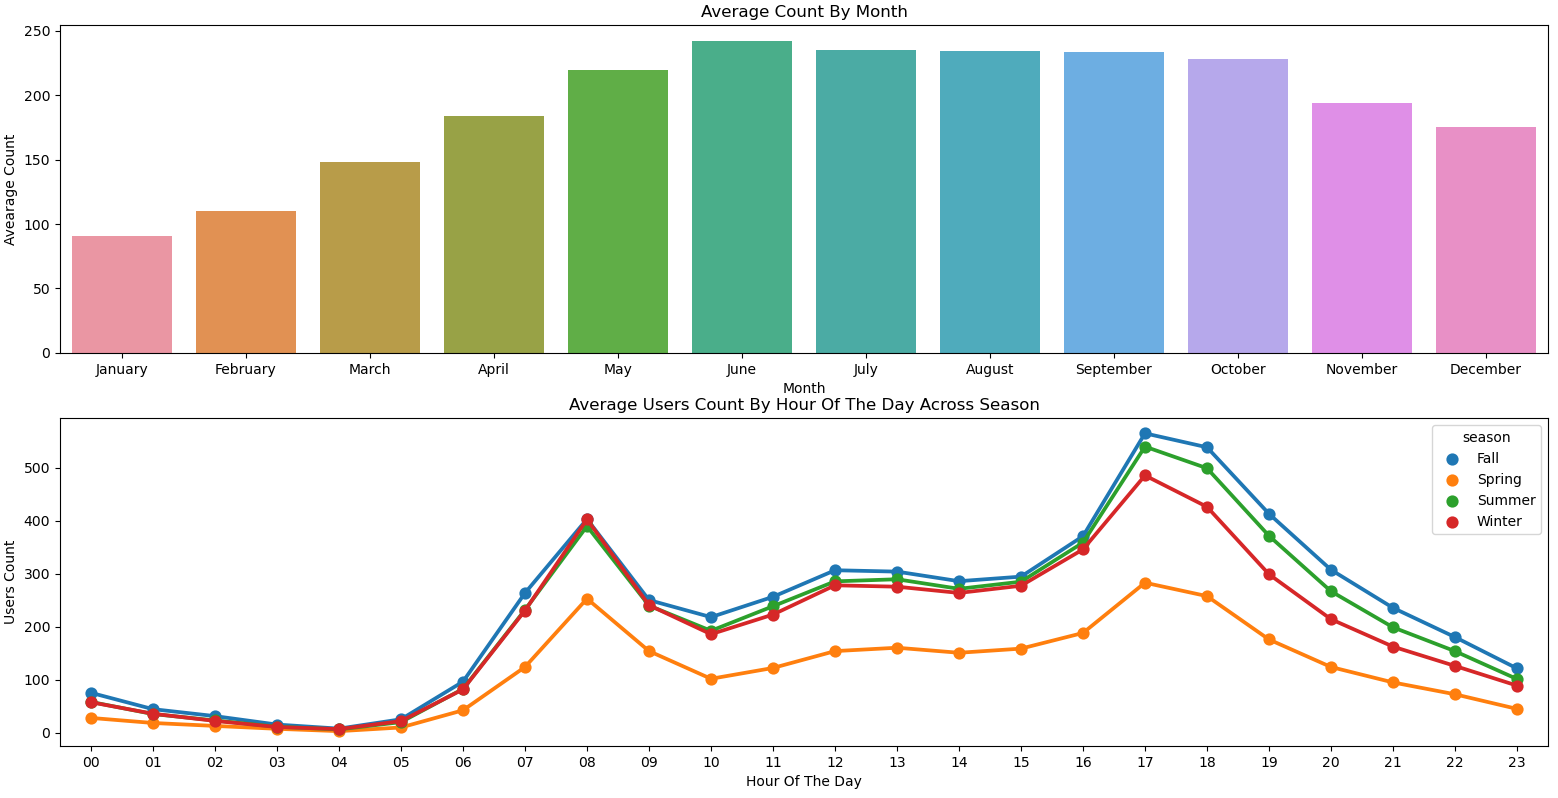
\includegraphics[scale=0.3]{./figure/Figure_6.eps}
	\caption{Visualizing Count I}
\end{figure}
3:On "Saturday" and "Sunday".More people tend to rent bicycle between 10AM and 4PM.\\
4:Registered user contribute the peak around 7AM-8AM and 5PM-6PM.
\begin{figure}[htbp]
	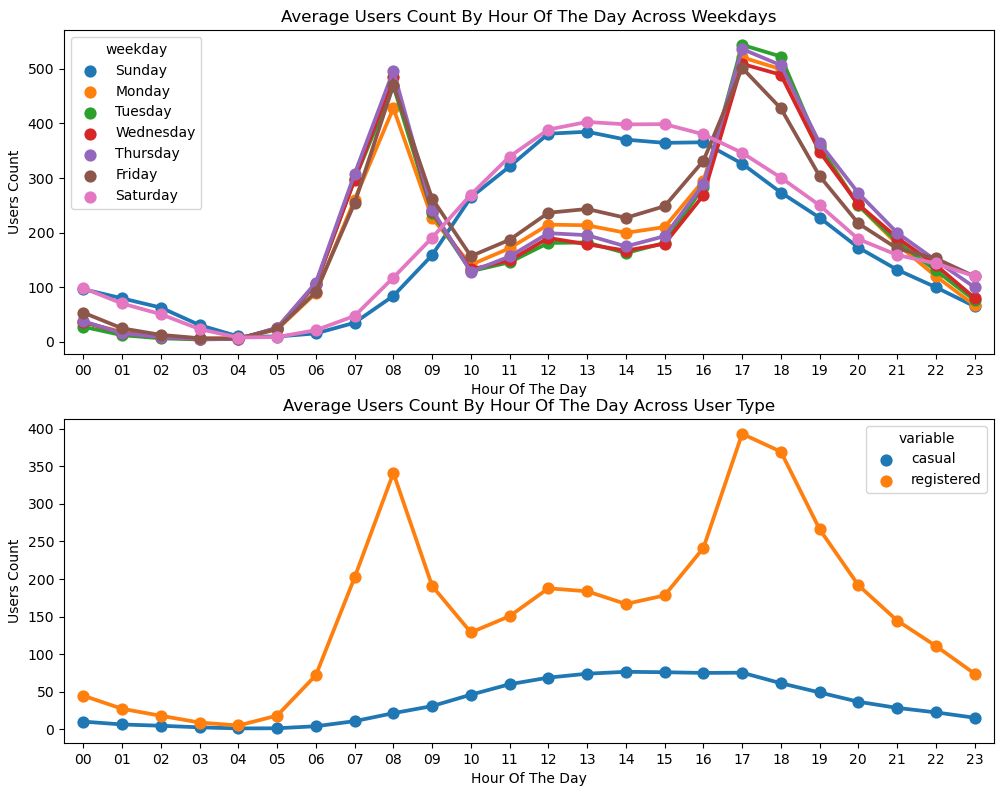
\includegraphics[scale=0.5]{./figure/Figure_7.eps}
	\caption{Visualizing Count II}
\end{figure}


\section{Feature Engineering and Model} \label{sec-method}
\subsection{Feature Processing}
Split the given date into "date, hour, year, weekday, month".
\begin{figure}[htbp]
	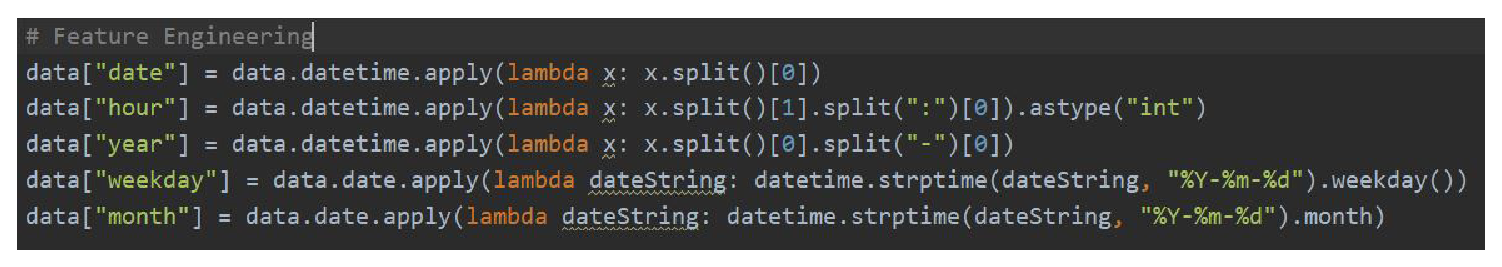
\includegraphics[scale=0.5]{./figure/1.eps}
	\caption{Time feature processing}
\end{figure}
According to visual analysis, select features that have strong correlation with count.
\begin{figure}[htbp]
	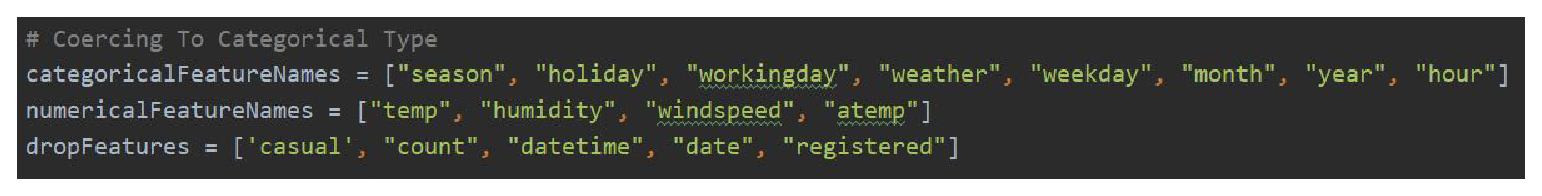
\includegraphics[scale=0.5]{./figure/2.eps}
	\caption{Feature selection}
\end{figure}

\subsection{Splitting train and test date}
Divide train set and test set according to whether there is count attribute.
\begin{figure}[htbp]
	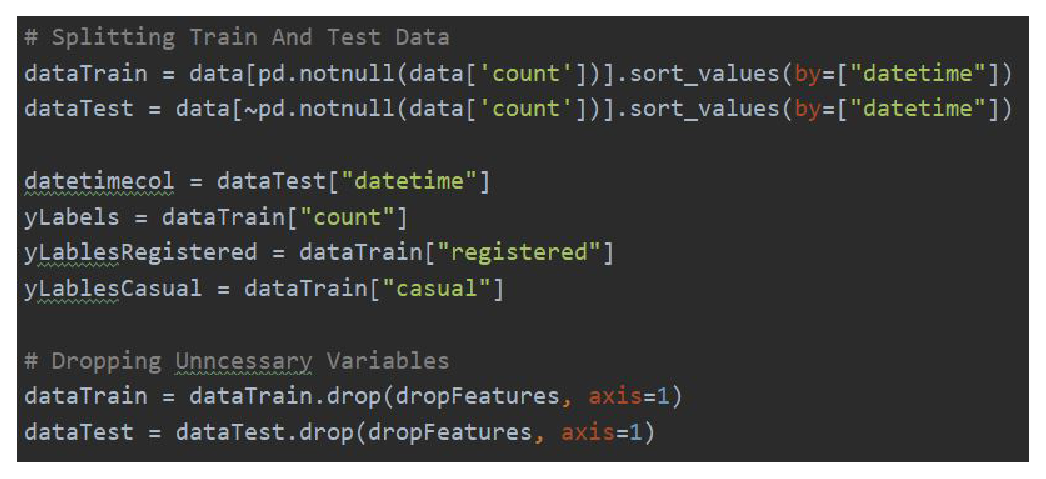
\includegraphics[scale=0.6]{./figure/3.eps}
	\caption{Training set and test set division}
\end{figure}

\subsection{Model}
I have choose the Ensemble Model - Gradient Boost. Compare the distribution of train and test results.It confirms visually that the model has not predicted really bad and not suffering from major overfitting problem.
\begin{figure}[htbp]
	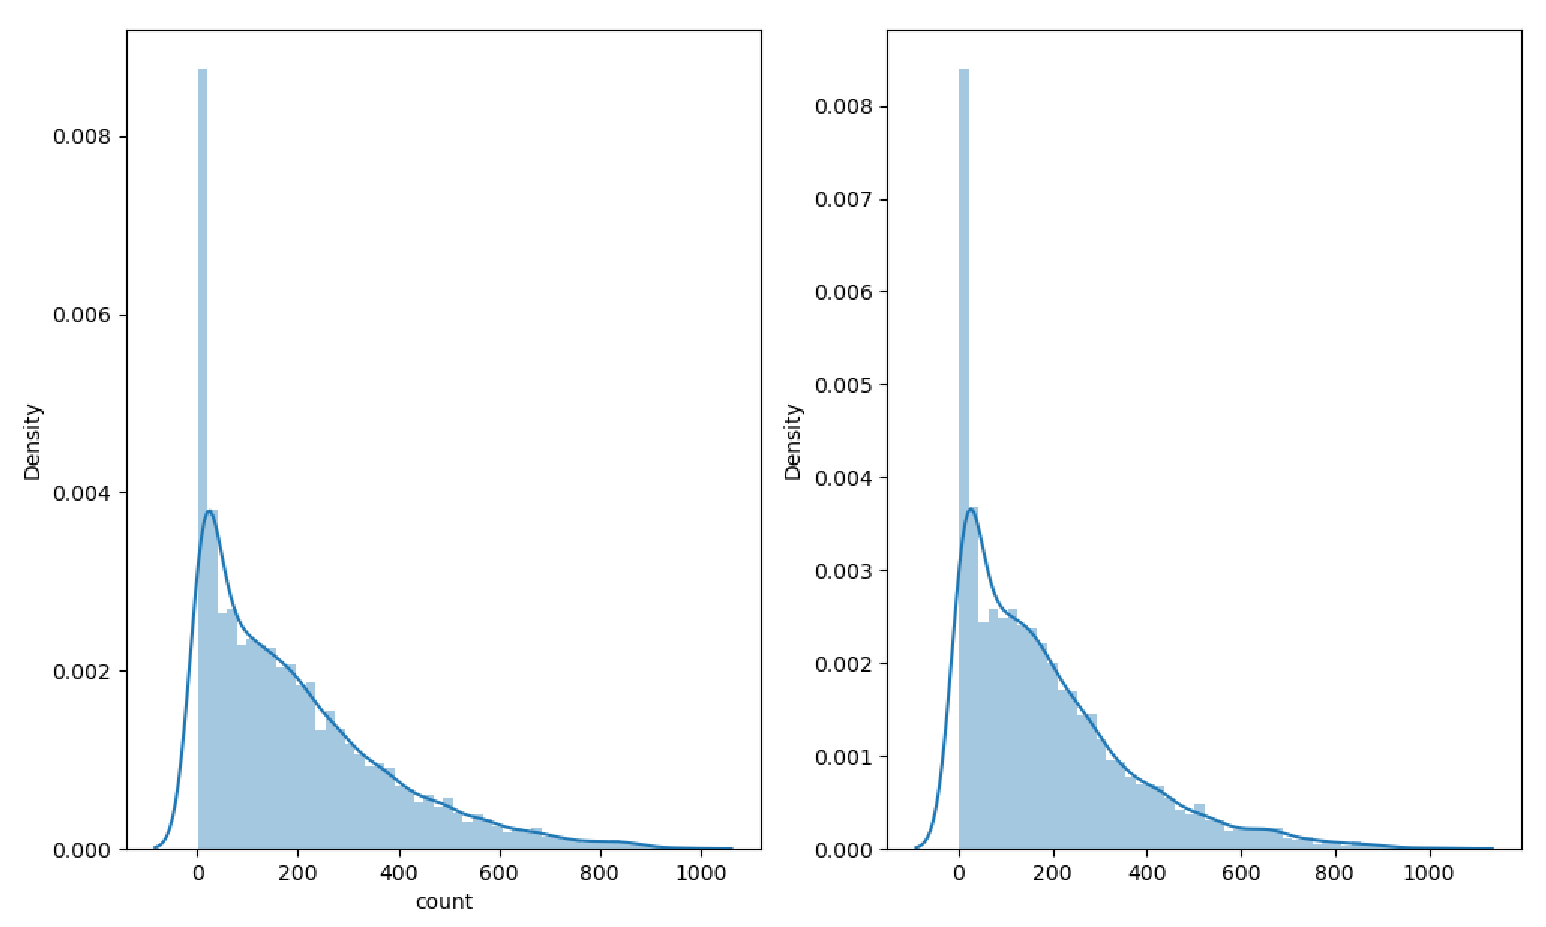
\includegraphics[scale=0.4]{./figure/models_Figure_1.eps}
	\caption{Distribution of train and test results}
\end{figure}

\section{Conclusions} \label{sec-conclusions}
Using RMSLE to calculate the error, it penalizes under-prediction even more.\\
RMSLE Value For Gradient Boost:  0.189973542608\\
The score of my submission in kaggle is 0.41867. Ranked 428 among 3242 teams.\\

As the result shows the model can effectively predict the count demand of bike. By solving this prediction problem, I am more familiar with python visualization and have a guiding idea for the data processing process. The learning task of the first stage was completed well.


%\section*{Acknowledgement}

%\lipsum[1]


%The authors would like to thank \ldots


%=================================================================
\section{Introduction}\label{sec-intro}

\subsection{Background}
The bicycle sharing system is a way of renting bicycles. Through the network of kiosk locations throughout the city, membership is automatically obtained, and the process of renting and returning bicycles. Using these systems, people can rent a bicycle from one place and return it to other places as needed. Currently, there are more than 500 bike sharing programs worldwide.\\

\subsection{Target}
In this competition, participants are asked to combine historical usage patterns with weather data in order to forecast bike rental demand in the Capital Bikeshare program in Washington, D.C.

\section{Data} \label{sec-preliminaries}
\subsection{Data Description}
The competition provide hourly rental data spanning two years.the training set is comprised of the first 19 days of each month, while the test set is the 20th to the end of the month. The taskis to predict the total count of bikes rented during each hour covered by the test set, using only information available prior to the rental period.\\

\begin{itemize}
	\smallskip
	\item \textbf{train.csv} -- it contains 10886 rows and 12 columns. Each row represents bike rental data for a certain hour. Each column indicates the current conditions
	\smallskip
	\item \textbf{test.csv} -- it contains 6493 rows and 9 columns. Compared with the train data, there are fewer "casual","registered" and "count" columns.
	\smallskip
	\item \textbf{sampleSubmission.csv} -- it clarifies the data submission format. It just contains 2 columns that is "datetime" and "count".
\end{itemize}

\subsection{Data Fields}
The following is a detailed introduction of the data \DIFaddbegin \DIFadd{for each attributes}\DIFaddend .\\
\begin{tabular}{c| c c c c }
	\toprule
	\textbf{column} & \textbf{description}  \\
	\midrule
	$datetime$ &  {hourly date + timestamp }\\
	$season$ &  {1 = spring, 2 = summer, 3 = fall, 4 = winter} \\
	$holiday$ &  {whether the day is considered a holiday} \\
	$workingday$ &  {whether the day is neither a weekend nor holiday} \\
	$weather$ &  {1=clear, 2=mist + cloudy, 3=light snow, 4=heavy rain} \\
	$temp$ & {temperature in Celsius} \\
	$atemp$ & {"feels like" temperature in Celsius} \\
	$humidity$ & {relative humidity} \\
	$windspeed$ & {wind speed} \\
	$casual$ & {number of non-registered user rentals initiated} \\
	$registered$ & {number of registered user rentals initiated} \\
	$count$ & {number of total rentals} \\
	\bottomrule
\end{tabular}

\subsection{Missing Values Analysis}
I use "missingno" to \DIFdelbegin \DIFdel{look }\DIFdelend \DIFaddbegin \DIFadd{visualize }\DIFaddend missing value in the dataset, Luckily the dataset do \DIFaddbegin \DIFadd{not }\DIFaddend has any missing value.\\
\begin{figure}[htbp]
	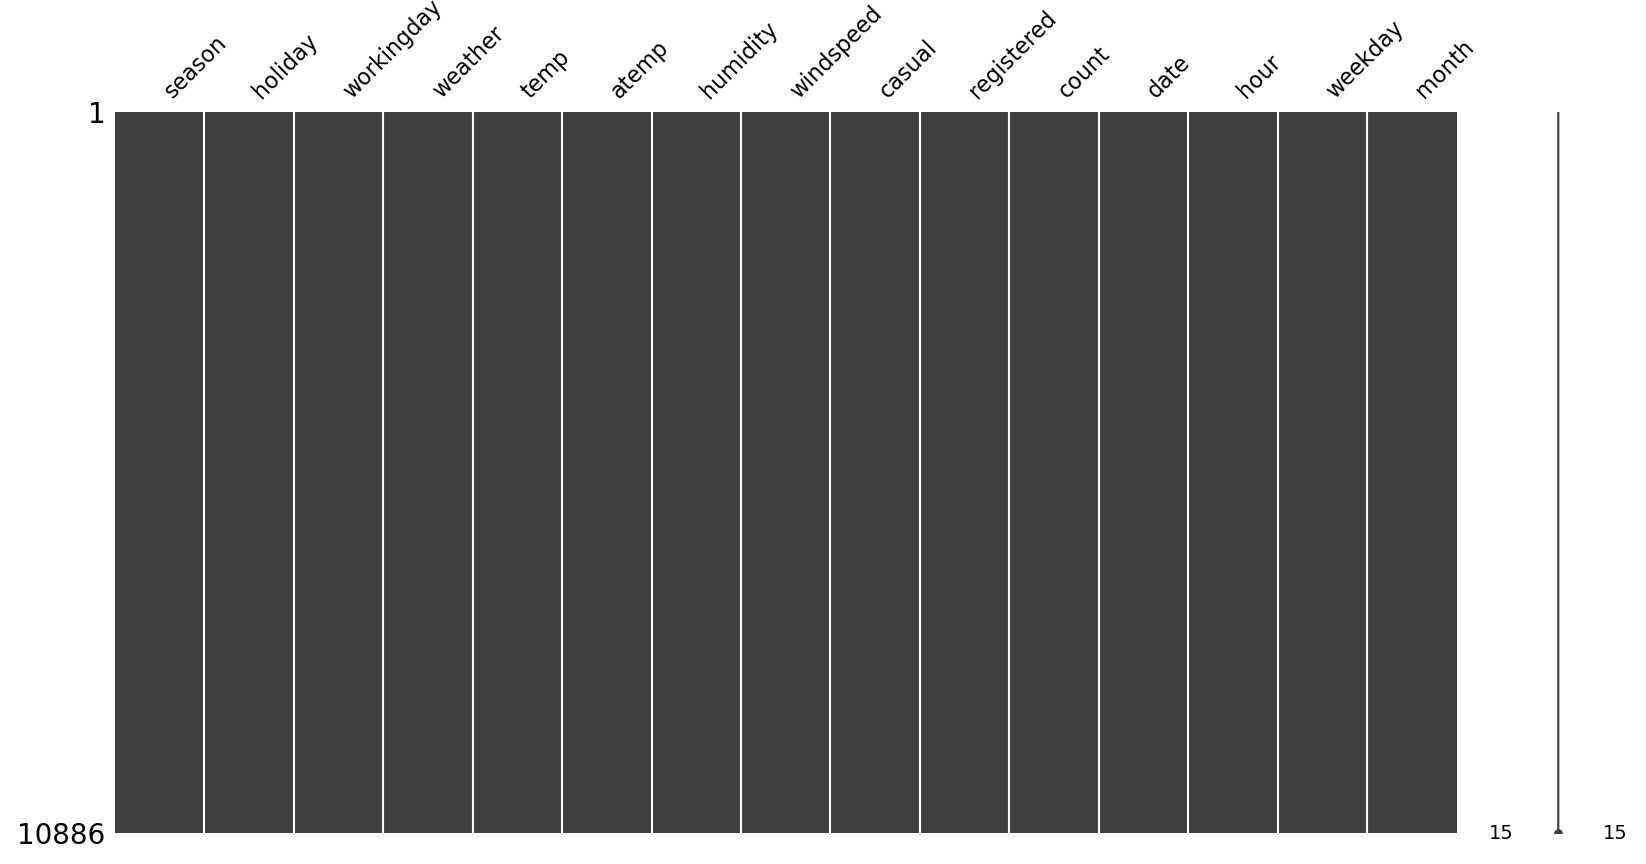
\includegraphics[scale=0.3]{./figure/Figure_1.eps}
	\caption{Missing values analysis}
\end{figure}

\subsection{Outliers Analysis}
1:Spring season has got relatively lower count. \\
2:The boxplot with "Hour Of The Day" is quiet interesting.The median value are relatively higher at 7AM to 8AM and 5PM to 6PM.\\
3:Most of the outlier points are mainly contributed from "Working Day" than "Non Working Day". 
\begin{figure}[htbp]
	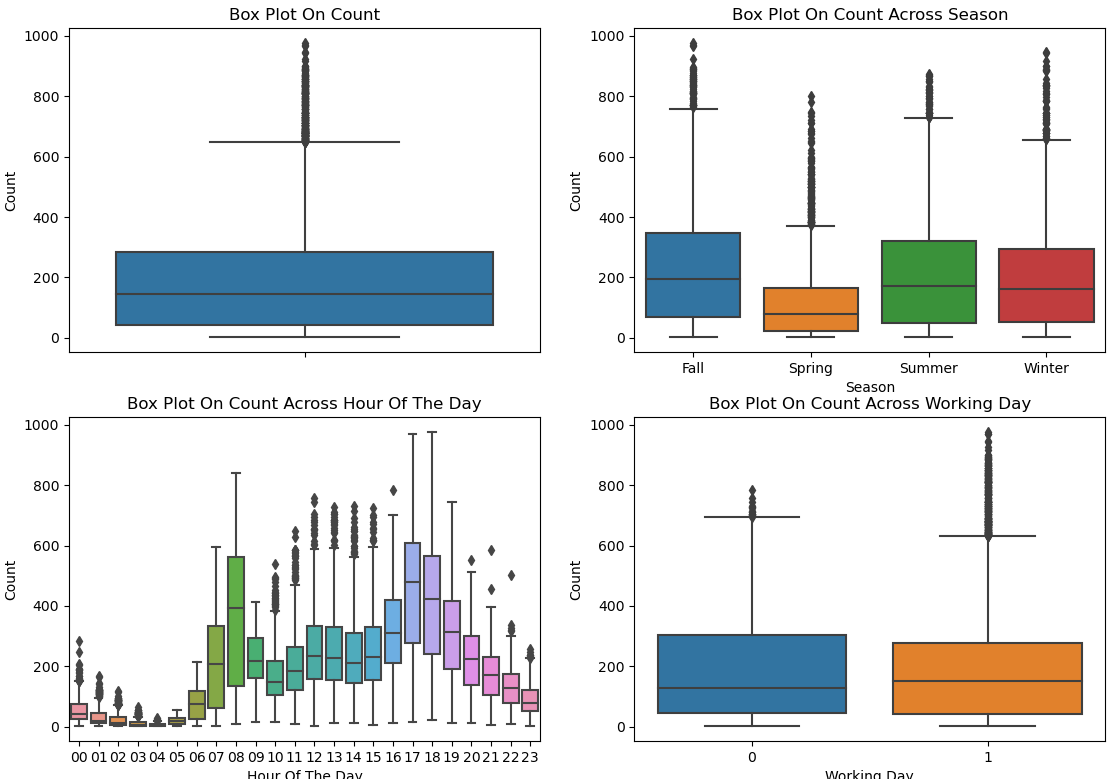
\includegraphics[scale=0.4]{./figure/Figure_2.eps}
	\caption{Outliers analysis}
\end{figure}

\subsection{Correlation Analysis}
1:temp and humidity features has got positive and negative correlation with count respectively. the count variable has got little dependency on "temp" and "humidity". \\
2:"Casual" and "Registered" are also not taken into account since they are leakage variables in nature and need to dropped during model building. \\
3:windspeed is not gonna be really useful numerical feature.
\begin{figure}[htbp]
	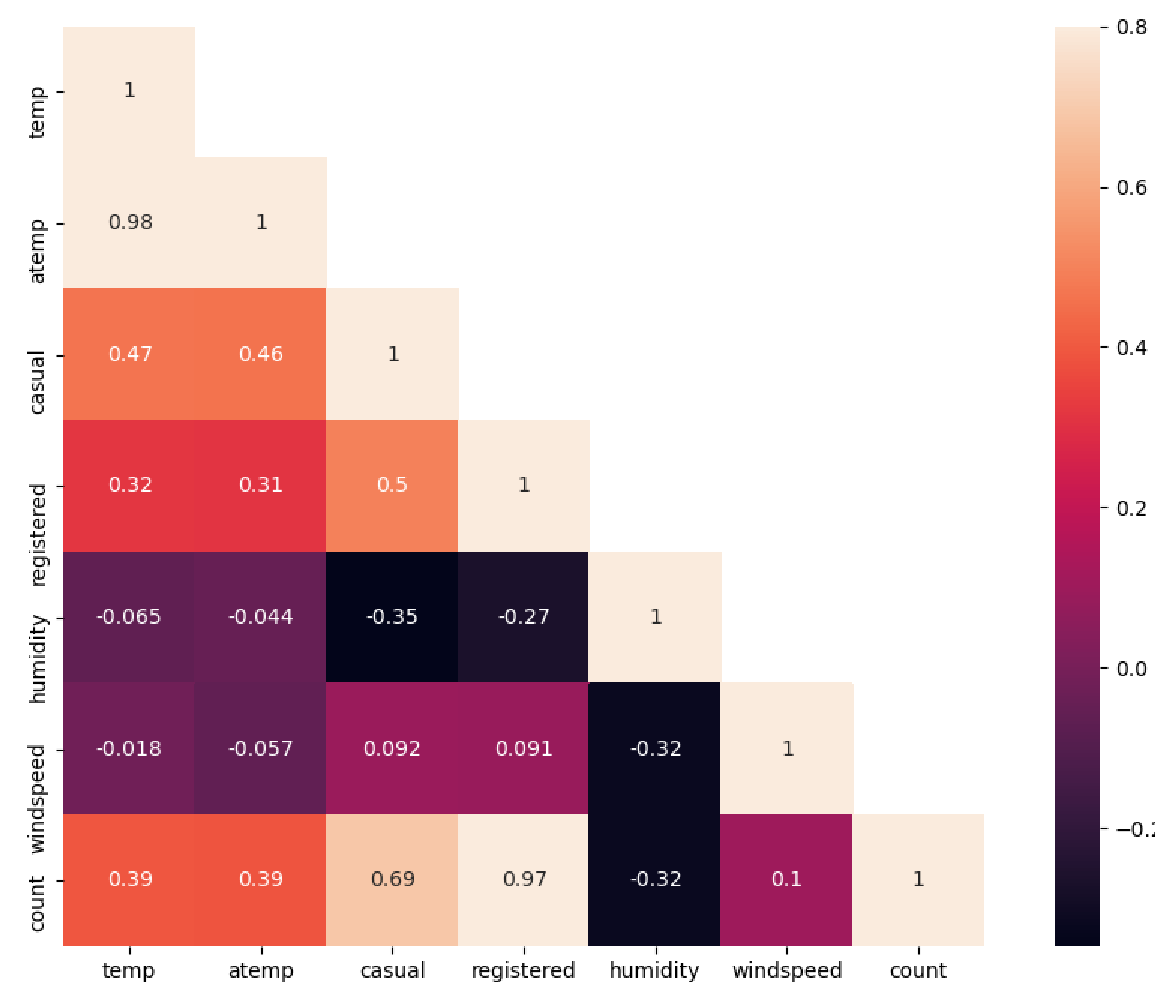
\includegraphics[scale=0.5]{./figure/Figure_3.eps}
	\caption{Correlation Analysis I}
\end{figure}

Regression plot in seaborn is one useful way to depict the relationship between two features. Here we consider "count" vs "temp", "humidity", "windspeed".
\begin{figure}[htbp]
	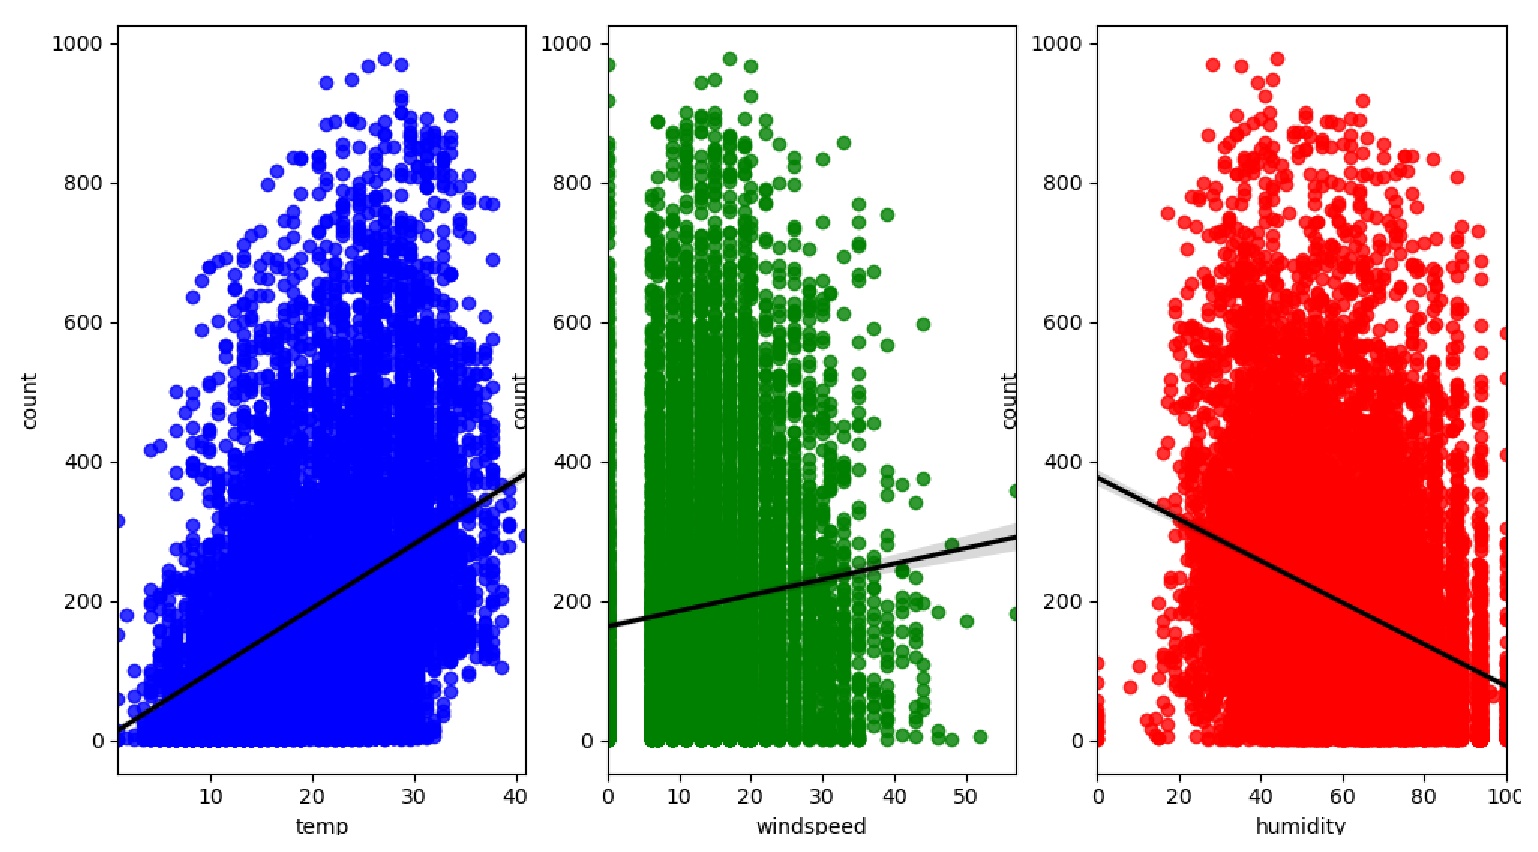
\includegraphics[scale=0.5]{./figure/Figure_4.eps}
	\caption{Correlation Analysis II}
\end{figure}

\subsection{Visualizing Distribution Of Data}
It is desirable to have Normal distribution \DIFdelbegin \DIFdel{deeplearning }\DIFdelend \DIFaddbegin \DIFadd{as most of the machine learning techniques }\DIFaddend require dependent variable to be Normal. One possible solution is to take log transformation on "count" variable after removing outlier data points.
\begin{figure}[htbp]
	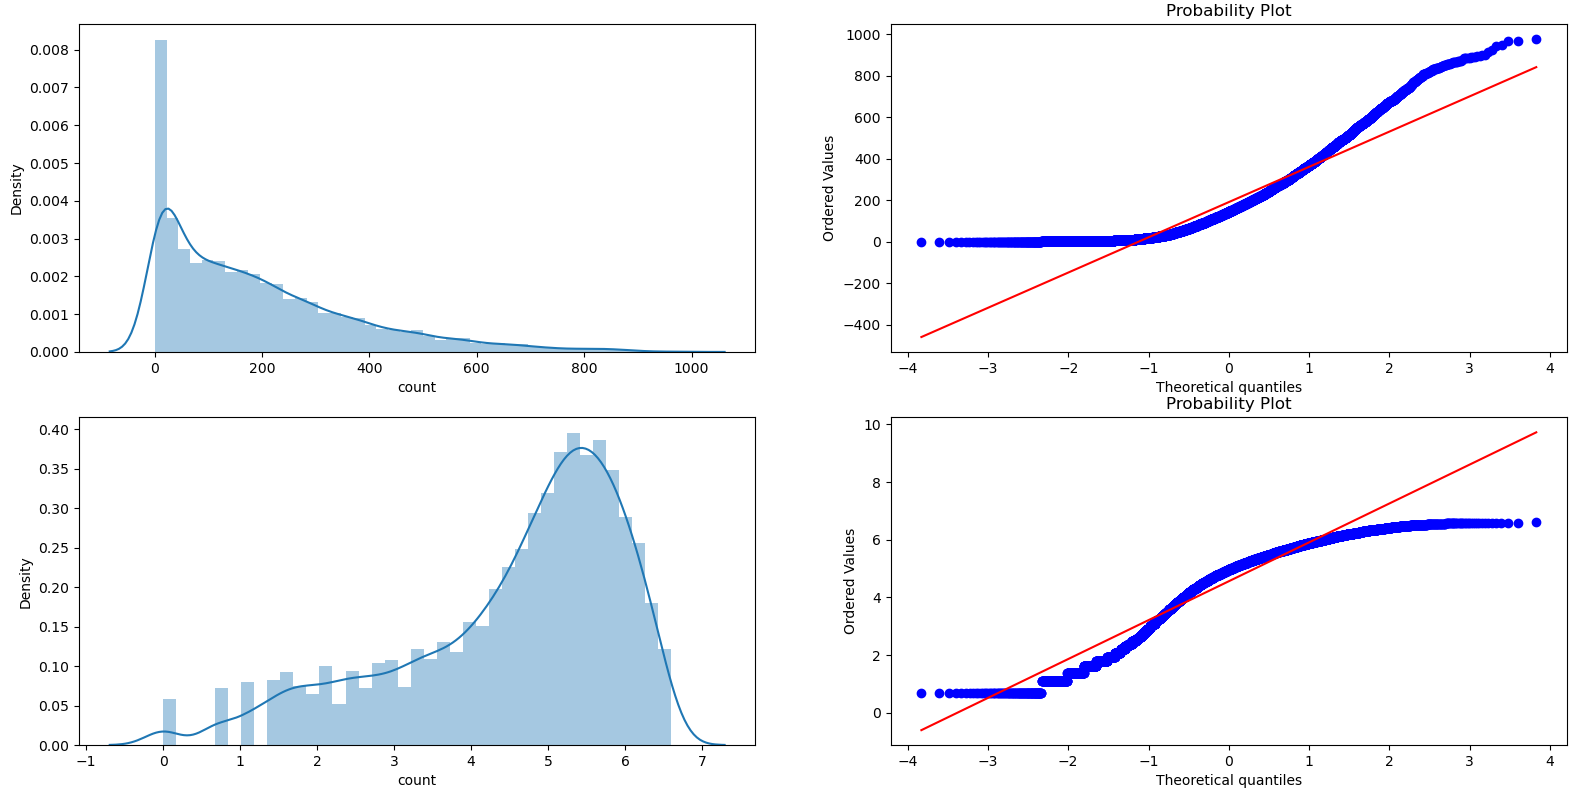
\includegraphics[scale=0.3]{./figure/Figure_5.eps}
	\caption{Visualizing Distribution Of Data}
\end{figure}

\subsection{Visualizing Count}
1:It is quiet obvious that people tend to rent bike during summer season. Therefore June, July and August has got relatively higher demand for bicycle.\\
2:On weekdays more people tend to rent bicycle around 7AM-8AM and 5PM-6PM. 
\begin{figure}[htbp]
	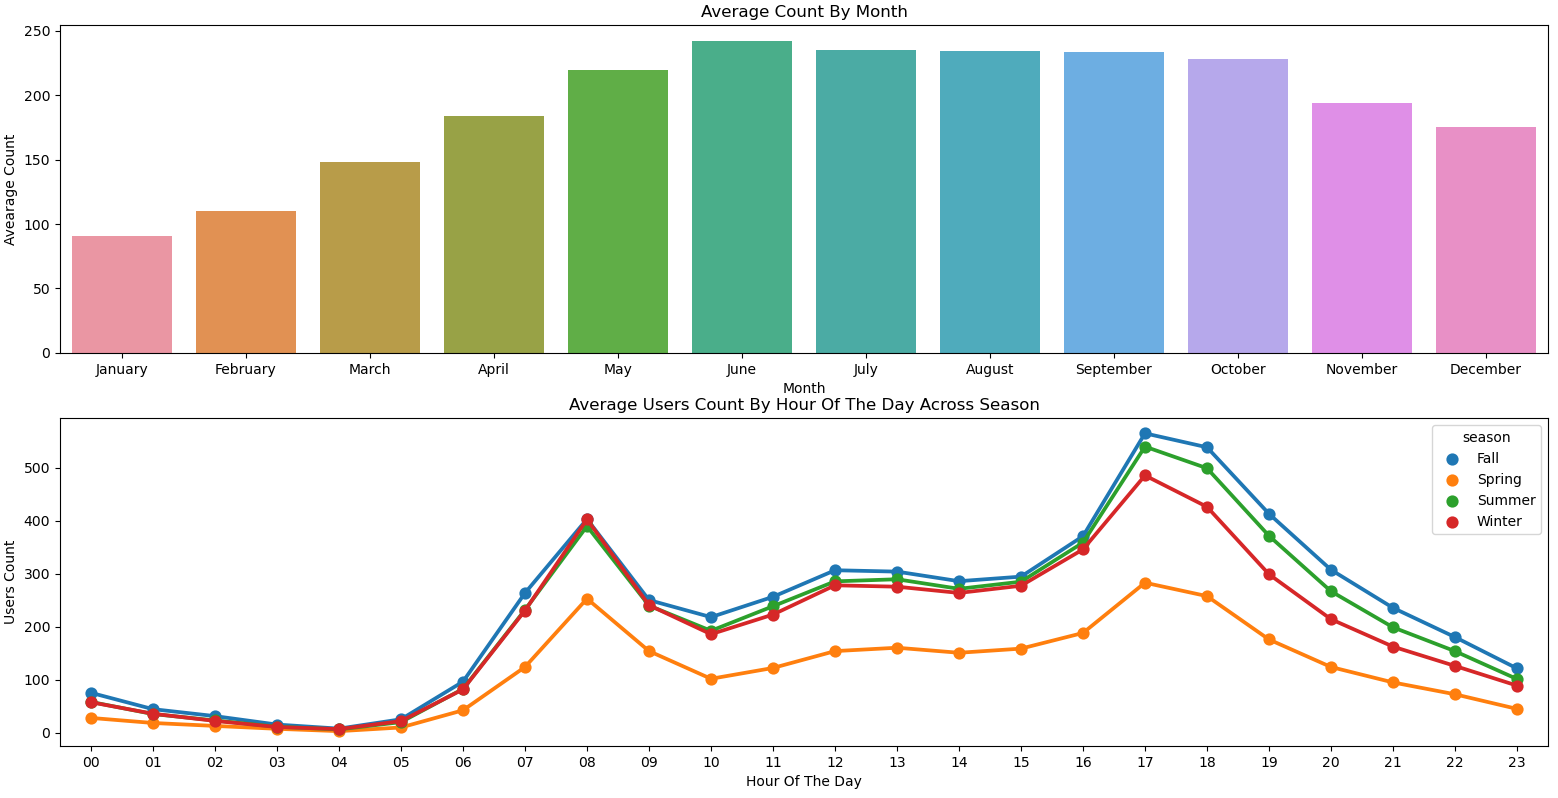
\includegraphics[scale=0.3]{./figure/Figure_6.eps}
	\caption{Visualizing Count I}
\end{figure}
3:On "Saturday" and "Sunday".More people tend to rent bicycle between 10AM and 4PM.\\
4:Registered user contribute the peak around 7AM-8AM and 5PM-6PM.
\begin{figure}[htbp]
	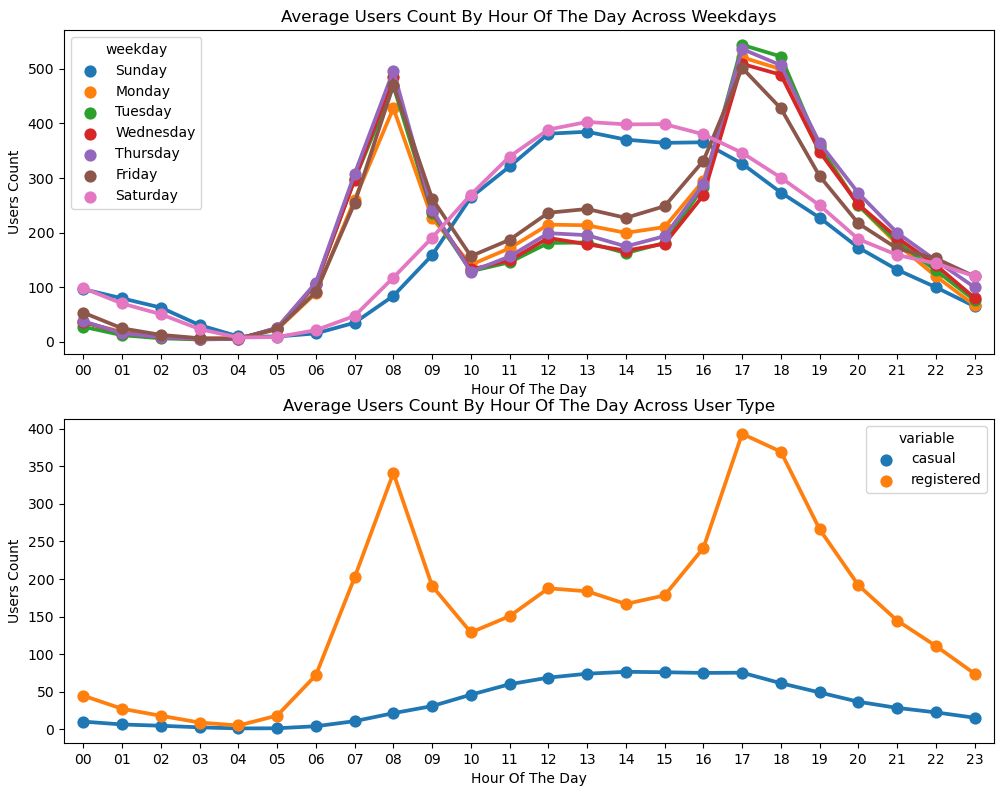
\includegraphics[scale=0.5]{./figure/Figure_7.eps}
	\caption{Visualizing Count II}
\end{figure}


\section{Feature Engineering and Model} \label{sec-method}
\subsection{Feature Processing}
Split the given date into "date, hour, year, weekday, month".
\begin{figure}[htbp]
	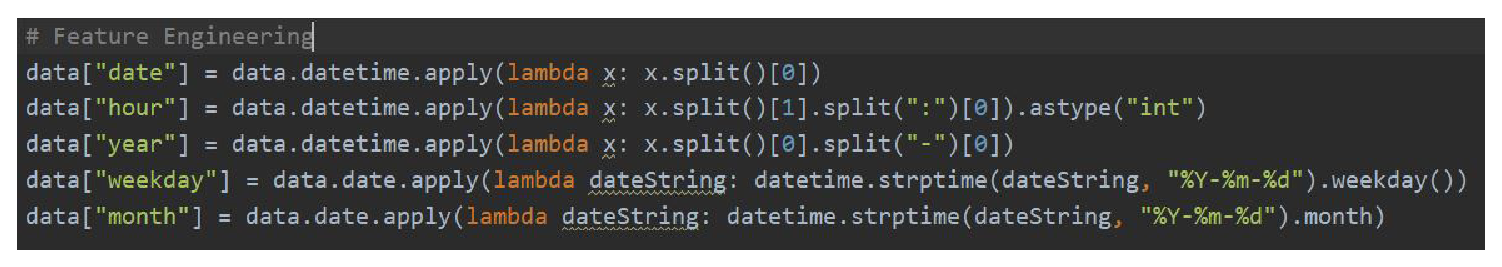
\includegraphics[scale=0.5]{./figure/1.eps}
	\caption{Time feature processing}
\end{figure}
According to visual analysis, select features that have strong correlation with count.
\begin{figure}[htbp]
	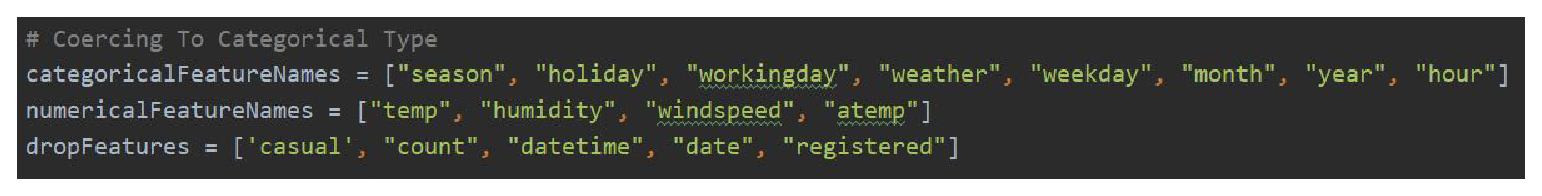
\includegraphics[scale=0.5]{./figure/2.eps}
	\caption{Feature selection}
\end{figure}

\subsection{Splitting train and test date}
Divide train set and test set according to whether there is count attribute.
\begin{figure}[htbp]
	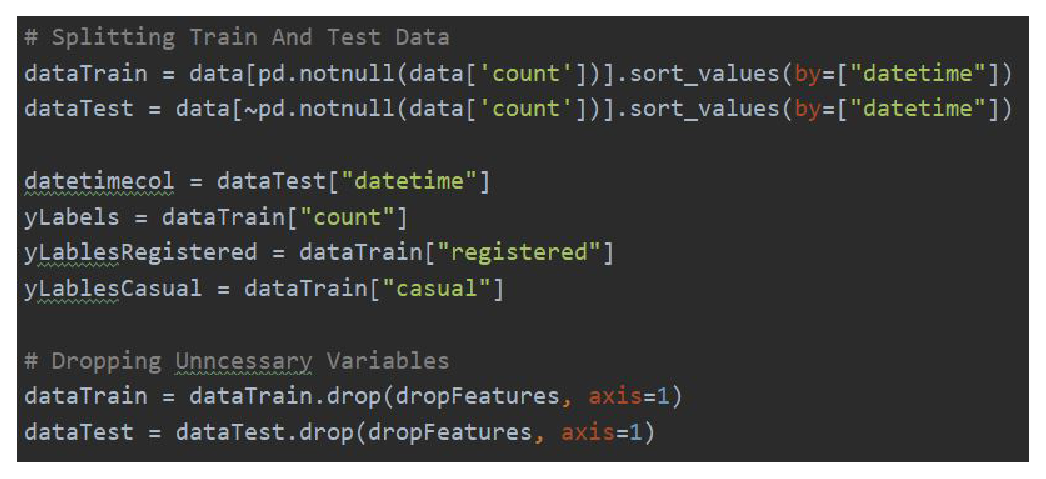
\includegraphics[scale=0.6]{./figure/3.eps}
	\caption{Training set and test set division}
\end{figure}

\subsection{Model}
I have choose the Ensemble Model - Gradient Boost. Compare the distribution of train and test results.It confirms visually that the model has not predicted really bad and \DIFdelbegin \DIFdel{do not have }\DIFdelend \DIFaddbegin \DIFadd{not suffering from major }\DIFaddend overfitting problem.
\begin{figure}[htbp]
	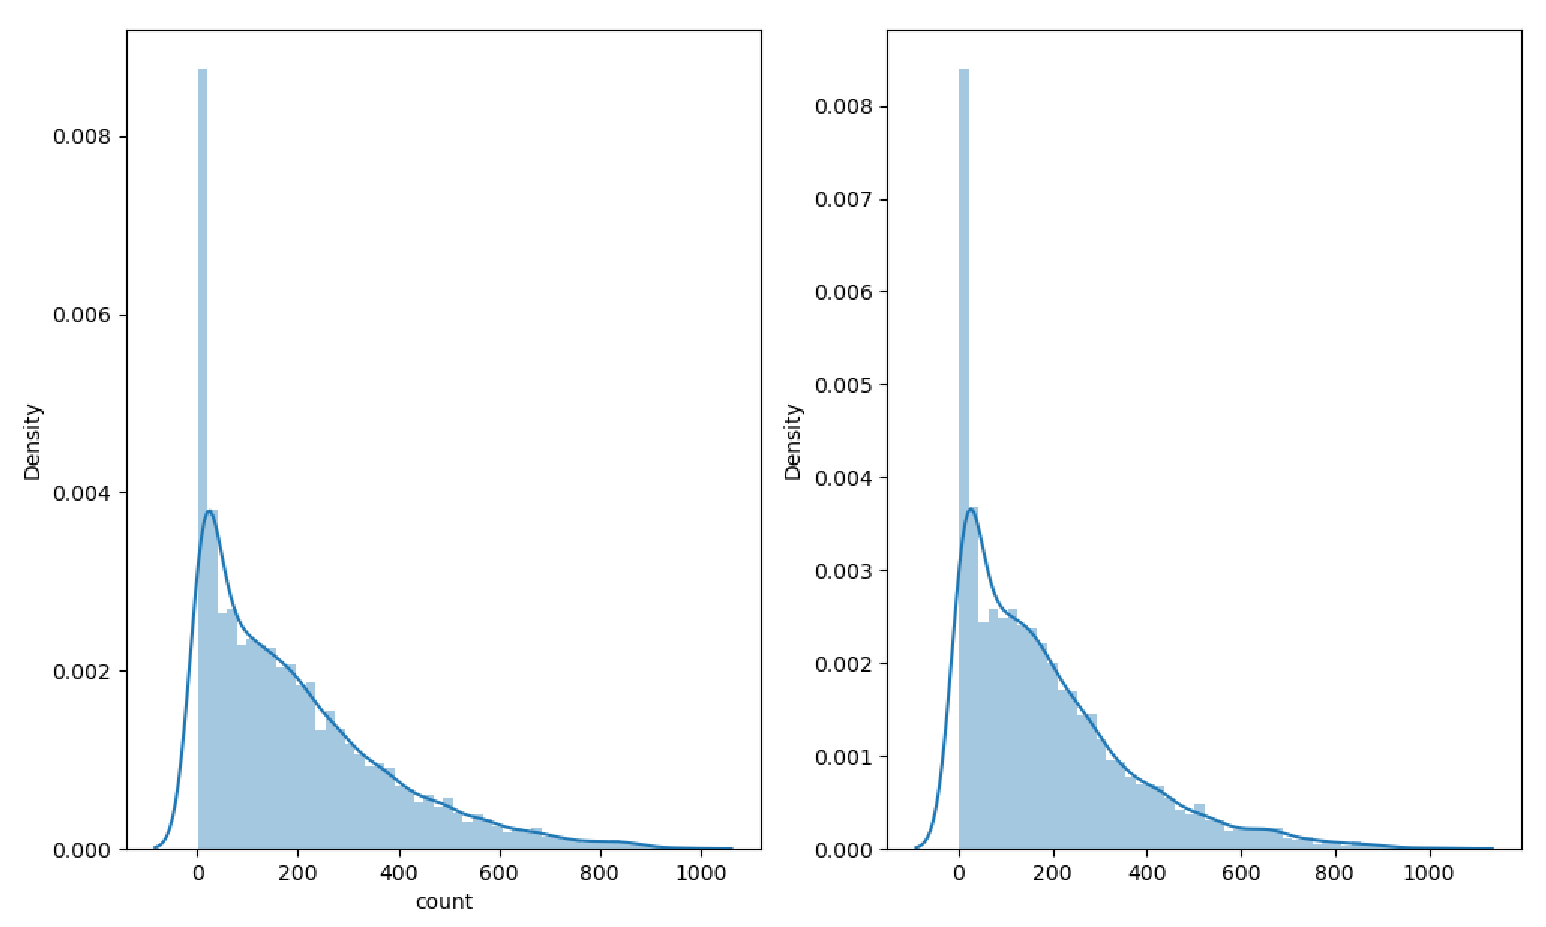
\includegraphics[scale=0.4]{./figure/models_Figure_1.eps}
	\caption{Distribution of train and test results}
\end{figure}

\section{Conclusions} \label{sec-conclusions}
Using RMSLE to calculate the error, it penalizes under-prediction even more.\\
RMSLE Value For Gradient Boost:  0.189973542608\\
The score of my submission in kaggle is 0.41867. Ranked 428 among 3242 teams.\\

As the result shows the model can effectively predict the count demand of bike. By solving this prediction problem, I am more familiar with python visualization and have a guiding idea for the data processing process. The learning task of the first stage was completed well.


%\section*{Acknowledgement}

%\lipsum[1]


%The authors would like to thank \ldots


% ----------------------------------------------------------------
\newpage
\bibliography{tuliplab,yourbib}
% TODO: you should change this yourbib into a proper bib file name
\bibliographystyle{plainnat}
%=================================================================

%\listoftodos

\end{document}

